\begin{figure}[h]

    \centering
    \renewcommand{\arraystretch}{2}
    
    \begin{tabular}{c c c c c}
    	
    {} & {} & {} & {} & {} \\
    
    {} & {} & {} & \multirow{2}{*}{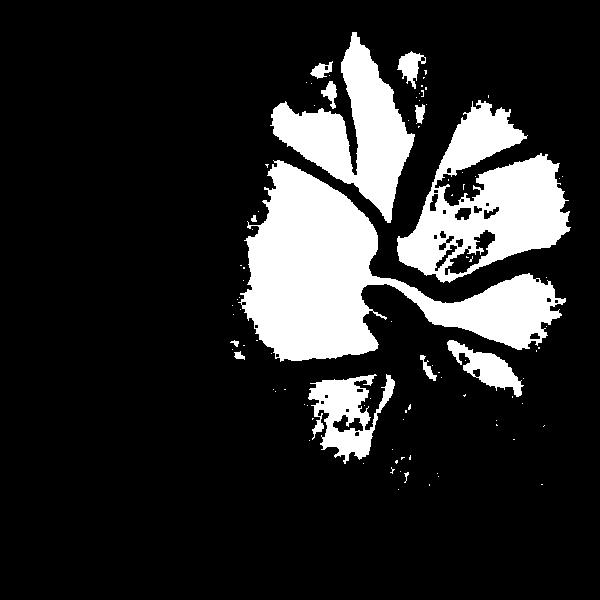
\includegraphics[width=2.5cm]{Images/Results/Segmentation/drishti101/2_cup.png}}{(c)} & 
    \multirow{2}{*}{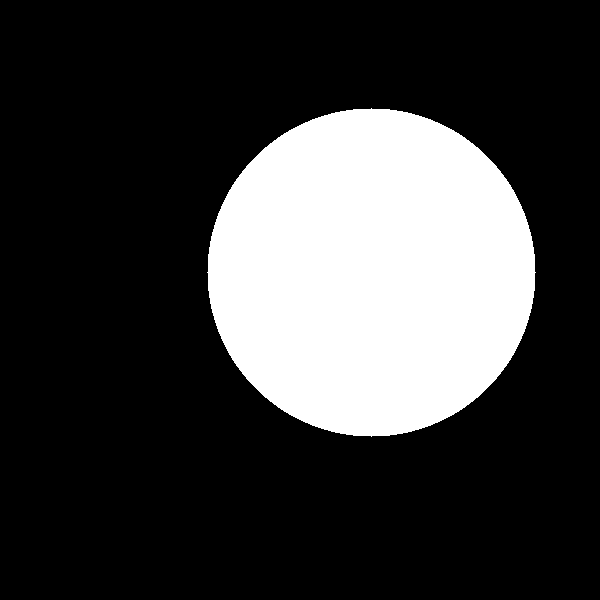
\includegraphics[width=2.5cm]{Images/Results/Segmentation/drishti101/6_hough_cup.png}}{(e)} \\
    
    {(2)} & \multirow{2}{*}{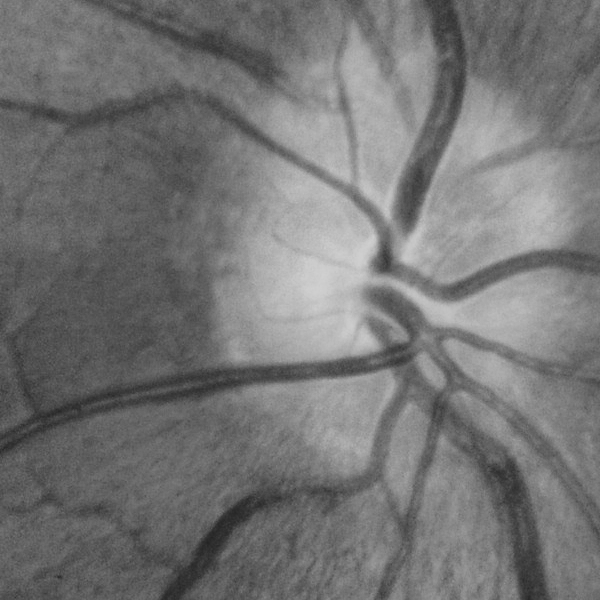
\includegraphics[width=2.5cm]{Images/Results/Segmentation/drishti101/0_crop.png}}{(a)} & 
    \multirow{2}{*}{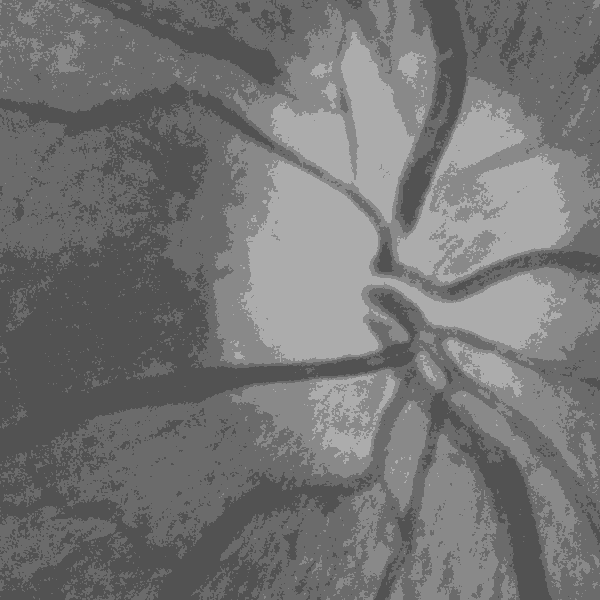
\includegraphics[width=2.5cm]{Images/Results/Segmentation/drishti101/1_kmeans.png}}{(b)} & {} & {} \\
    
    {} & {} & {} & \multirow{2}{*}{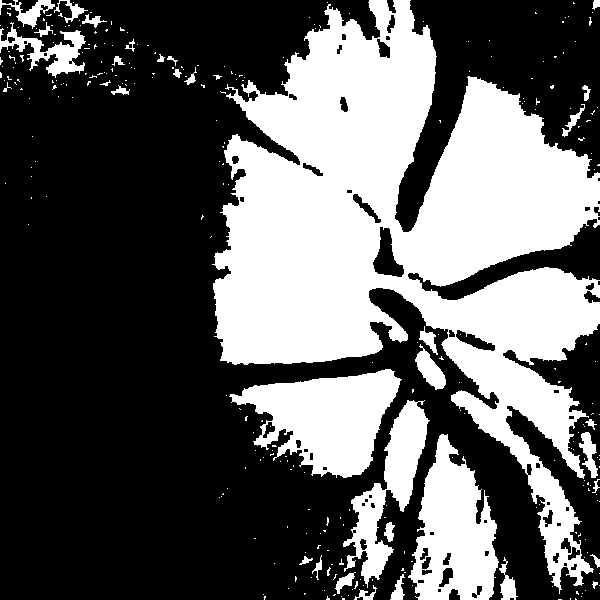
\includegraphics[width=2.5cm]{Images/Results/Segmentation/drishti101/3_do.png}}{(d)} & 
    \multirow{2}{*}{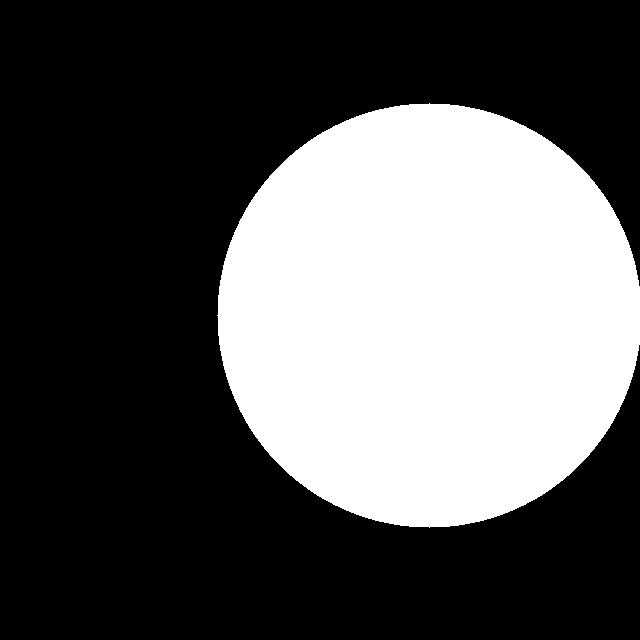
\includegraphics[width=2.5cm]{Images/Results/Segmentation/drishti101/7_hough_do.png}}{(f)} \\
    
    {} & {} & {} & {} & {} \\
    
    \end{tabular}

\caption{\label{segmentation_results_failures}OC and OD segmentation failure: (a) sub-image around the OD, (b) k-means clustering (K=4), (c) OC and OD extraction, (d) final segmentation with circular Hough transform, (). The resulting segmentation lead to underestimated regions.}

\end{figure}